
%%%%%%%%%%%%%%%%%%%%%
\section{Définitions}
%%%%%%%%%%%%%%%%%%%%%
%
%\subsection{Ondes et particules}
\subsection{Lumière et matière}

Une particule est un "grain de matière". Le mouvement d'une particule est décrit par sa position en fonction du temps. Au cours de son mouvement, une particule conserve sa nature ponctuelle.

%Une particule peut être considérée peut supposer les particules ponctuelles (leur taille est petite).
%. Ce mouvement peut se traduire comme un transfert d'énergie
%Une onde est un transfert d'énergie sans transport de matière.

Une onde a besoin d'un milieux matériel pour se propager. Le mouvement de l'onde consiste en une déformation du milieux. Une onde est nécessairement étendue dans l'espace, au cours de son mouvement, elle subit une déformation, sa "forme" change au cours de son mouvement.

%Le mouvement d'une onde est décrit par la donnée de son "amplitude".

Décrire la matière comme constituée de particules revient à supposer qu'elle a une nature granulaire : la matière n'est pas divisible à l'infini, il existe une limite où l'on observe des grains indivisibles, des particules élémentaires. Cette description s'oppose à une vision "continue" de la matière.

\subsubsection{Exemples}

Dans le cas des ondes sonnores, le milieux de propagation est l'air. Dans le cas des ondes sismiques, le milieux de propagation est la Terre. Les vagues dans la mer sont qualifiées d'ondes de surfaces.

\vspace{0.5cm}
\begin{minipage}[c]{.45\linewidth}

%%%%%%%%%%%%%%%%%%%%%        PERSONNAGE AU BORD D'UNE MARE
%  DÉFINITIONS

\tikzset{
  feuillage/.style = {decoration={random steps, segment length=0.4mm}, decorate},
  tronc/.style   = {decoration={random steps, segment length=2mm, amplitude=0.2mm}, decorate}}

\tikzset{  arbre/.pic={ \foreach \w/\f in {0.3/30,0.2/50,0.1/70} { \fill [brown!\f!black, tronc] (-\w/2,0) rectangle +(\w,3); } \foreach \n/\f in {1.4/40,1.2/50,1/60,0.8/70,0.6/80,0.4/90} { \fill [green!\f!black, feuillage](0,3) ellipse (\n/1.5 and \n); }}}

\tikzset{  personnage/.pic={ { \fill [black] (0,0)ellipse(0.25 and 0.55); } 
  { \fill [black](0,0.75)circle(0.2); }
    % jambe et pieds
  {\fill [rounded corners=2pt] (0.1,-0.3)rectangle(-0.1,-1.5);}
  {\fill [rounded corners=2pt] (0.3,-1.4)rectangle(-0.1,-1.5);}
    % bras
  {\fill [rounded corners=2pt, rotate=-15] (-0.1,0.42)rectangle(0.5,0.29);}
  {\fill [rounded corners=2pt] (0.44,0.17)rectangle(1,0.29);}}}

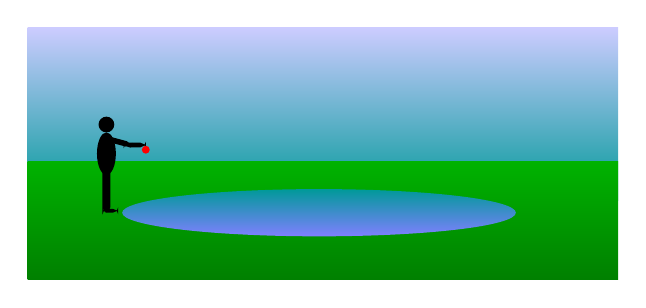
\begin{tikzpicture}%[scale=0.5]
    %  Ciel
  \shade[bottom color=cyan!60!black, top color=blue!20!white] (0,0) rectangle (7.5,2.2);
    %  Sol
  \shade[bottom color=green!50!black, top color=green!70!black] (0,0.5) rectangle (7.5,-1);
    %  Mare
  \shade[bottom color=blue!50!white, top color=cyan!60!black] (3.7,-0.15) ellipse (2.5 and 0.3);
    %  Arbre
 % \pic at (2,2)    {arbre};

    %  Personnage
  \begin{scope}[xshift=1 cm,yshift=0.6 cm]
    % corps et tête
 \fill [black] (0,0)ellipse(0.12 and 0.27);
 \fill [black](0,0.37)circle(0.1);
    % jambe et pieds
 \fill [rounded corners=2pt] (0.05,-0.15)rectangle(-0.05,-0.75);
 \fill [rounded corners=2pt] (0.15,-0.7)rectangle(-0.05,-0.75);
    % bras
 \fill [rounded corners=2pt, rotate=-15] (-0.1,0.22)rectangle(0.28,0.15);
 \fill [rounded corners=2pt] (0.22,0.08)rectangle(0.5,0.14);
   % Balle
 \fill[red] (0.5,0.05) circle(0.05);
  \end{scope}

\end{tikzpicture}

%%%%%%%%%%%%%%%%%%%%%%%%%%%%%%%%%%%%%%%%%%%%%%%%%%%%%%%%%%%%%%%%%%%%%%%%%%%%%%%%

\end{minipage}
\hfill
\begin{minipage}[c]{.45\linewidth}
Un expérimentateur laisse tomber une balle dans une mare. Lorsque la balle frappe la surface de l'eau, une onde circulaire est créée. On observe cette onde se propager dans la mare et atteindre l'autre rive.
%vers la rive opposé. Atteignant celle-ci, on observe une érosion.
\end{minipage}

%\subsubsection{Exemple microscopique}

%Les électrons sont des particules chargés électriquement.'interaction entre deux électrons

%
\subsection{Champs}

Un champs est la donnée d'une grandeur en tout point de l'espace.

\subsection{Quanton}
%
Un quanton n'est pas une onde et n'est pas un corpuscule. C'est un objet dont le mouvement est décrit par l'équation de schrödinger.

Un quanton se déplace comme une onde et se dévoile comme un corpuscule.

%%%%%%%%%%%%%%%%%%%%%%%%%%%%%%%%%%%%%%%%%%%%%%%%%%%%%%%%%%%%%%%%%%%%%%%%%%%%%%%%
